\documentclass[twocolumn]{svjour3}
\usepackage{siunitx}
\usepackage{graphicx}
\newcolumntype{L}{>{\centering\arraybackslash}m{1.7cm}}
\newcommand{\MYfooter}{\smash{
\hfil\parbox[t][\height][t]{\textwidth}{\centering
\thepage}\hfil\hbox{}}}
\usepackage{algorithmic}
\usepackage{multirow}
\usepackage{algorithm2e} 
\usepackage[english]{babel}
\usepackage[misc]{ifsym}
%\usepackage{aps-bibstyle}
\setlength{\textfloatsep}{0.1cm}
\let\proof\relax
%\usepackage{amsthm}
%\usepackage{caption}
\usepackage[authoryear]{natbib}
\newtheorem{definition1}{Definition}
\usepackage[hyphens]{url}
\usepackage[hidelinks]{hyperref}
\hypersetup{breaklinks=true}
\urlstyle{same}
\setlength{\bibhang}{2em}
\usepackage{etoolbox}

\makeatletter
\renewcommand\@biblabel[1]{\hspace*{\labelwidth}}
\apptocmd{\NAT@thebibliography}{\setlength\itemindent{-25pt}}{}{}
\makeatother



\begin{document}


\journalname{Journal of Ambient Intelligence \& Humanized Computing}

\title{WALE: A Weighted Adaptive Location Estimation Algorithm}
\author{Darshak Sundar \and Siddharth Sendil \and Vasanth Subramanian \and Vidhya Balasubramanian }
\authorrunning{Sundar et al.}
\institute{ Vidhya Balasubramanian (\Letter)  \\Dept of Computer Science and Engineering \\ Amrita School of Engineering, Coimbatore \\ Amrita Vishwa Vidyapeetham \\ India\\ \email{b\_vidhya@cb.amrita.edu}}

\titlerunning{WALE}

%\date{Received: date / Accepted: date}

\maketitle

\begin{abstract}
Indoor pervasive applications depend on reliable indoor localization solutions. Indoor localization using WiFi is gaining ubiquitous usage owing to its simplicity and inexpensiveness. A conventional method of localization is trilateration, which can be accomplished using signal strength or time of flight of a radio signal between receiver and transmitter. However, trilateration is prone to errors in accuracy that can occur due to various factors. A common reason for the failure of trilateration is due to the errors in distance estimation resulting in a poor quality of trilateration. In this paper, we propose a novel Weighted Adaptive Location Estimation (WALE) algorithm. The proposed WALE algorithm provides an accurate localization in comparison to trilateration by taking into account the quality and properties of the circle overlaps. Based on the overlap properties a distance re-estimation and classification of points based on whether they are trilaterable is performed. A maximum likelihood estimation over a weighted grid of this region provides the location estimate. Our experiments over real indoor test-beds have demonstrated that our algorithm provides high accuracies with high stability in comparison to other algorithms. We achieve high accuracies ranging from 1.20m to 2.20m in majority of the cases and an average of 2.98m in a large office space with a standard deviation of 1.65.

\keywords{Indoor Localization \and Trilateration \and Weighted Adaptive Trilateration \and WiFi Localization}

\end{abstract}


\section{\textbf{Introduction}}
In recent years, WiFi-based indoor positioning has garnered widespread interest from various communities because of the sheer number of applications it has and the myriad of problems it solves. It is an important component of disaster response systems, smart buildings, warehouses, commercial spaces designed to improve shopper experiences etc. To enable localization in any building with minimal infrastructural overhead, smart-phone based localization that uses WiFi is most suitable due to its pervasive availability and cost effectiveness \citep*{4796924}. This paper describes a novel and efficient WiFi localization technique that requires minimal infrastructure overhead and calibration, therefore making it robust for implementation in any smart building. 

Received Signal Strength (RSS) is the preferred parameter for such localization and signal strength based localization is an important area of research owing to its simplicity \citep*{RSSI_Analysis, Analysis_RSSI}. RSS-based localization techniques commonly depend upon fingerprint maps and these techniques have been proven to achieve precise locations in indoor environments \citep*{kaemarungsi2012analysis, zhang15, 4796924, Hossain20151}. However, generating a fingerprint is laborious and a tediously long process \citep*{ekahau, 4343996,4796924}. To alleviate this problem several approaches have been suggested including synthetically generating fingerprinting maps, crowd-based approaches for fingerprinting, etc. \citep*{4796924}. However, there is still a need to design better non- fingerprinting approaches to address scalability and robustness in large indoor spaces.

Multilateration is the most well known non- fingerprinting method for localization using RSS \citep*{yang2009indoor}. Multilateration uses a geometric approach, where the intersection of k-spheres corresponding to the influence of the k-nearest routers estimates the location of the receiver. Standard multilateration experiments in indoor spaces generally use trilateration. While the relative accuracy of trilateration compared to fingerprinting algorithms is poor, its ease of implementation makes it a candidate of interest. The labour involved in fingerprinting techniques and the low reliability offered by non-fingerprinting techniques, open up avenues for further research in improving the accuracy of trilateration and doing so will help make indoor localization more robust. 

In trilateration, since the intersection region is primarily dependent on the radii of the three circles, which in turn are reliant on a distance estimator, the localization accuracy is affected by the accuracy of the distance estimation method. Distance estimation methods use path loss models like the log-distance model, ITU, and Okamura-Hata \citep*{soorty2015finding}, and calculate distances based on RSS. However, the estimated distance is inaccurate since these models do not adequately account for obstacles dispersion, reflections etc in the indoor space. In order to reduce the error in trilateration, one option is to define a better indoor path loss model. This may be developed for specific environments, but is not generalizable, and cannot account for people movement and other dynamic factors that may affect RSS. There have been attempts to re-estimate the distance by accounting for obstacles \citep*{chandrasekaran2015inplace}. However, this is difficult in large scale environments with randomly placed obstacles and therefore looking at the trilateration pattern itself may give some clues.

The quality of trilateration is poor in many cases as evidenced by Figure \ref{fig:intro}, i.e, the intersection between circles is not always perfect. Many times circles do not intersect and in other times the percentage of intersection is large. This is caused either due to underestimation or overestimation of distances by the chosen path loss model. Additionally, certain points are located in positions where traditional trilateration contributes to higher error and can be classified as non-trilaterable.

\begin{figure}[!ht]
\centering
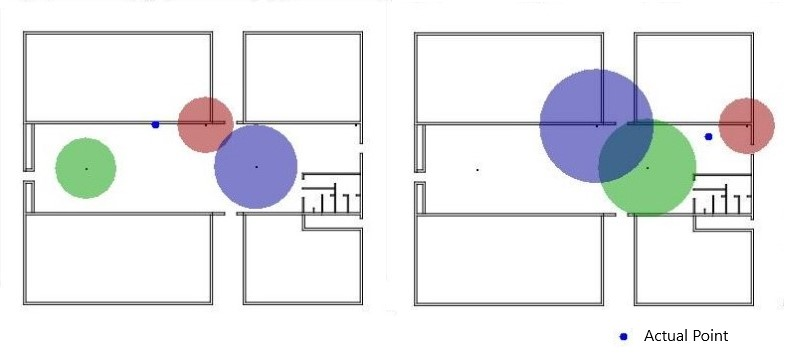
\includegraphics[width=90mm,height=40mm]{Intro_1.jpeg}
\centering\caption{Examples of poor Trilateration}
\label{fig:intro}
\end{figure}

Based on the determination of underestimation and overestimation from the trilateration pattern, the radii of the circles are recalculated. Location estimation after the circle re-sizing is performed using an adaptive weighting algorithm, which helps account for factors influencing the accuracy. This algorithm assigns different weights to points inside the circle, these weights correlate to the likely probability of the point lying in the estimated location. A maximum likelihood estimation over this weighted grid of this region provides the location estimate. 

The rest of the paper is organized as follows: section 3 explains our key observations based on our analysis of trilateration while section 4 describes in detail our adaptive localization algorithm. The experimental details and results are discussed in section 5 and finally, the last section concludes. The next section outlines the related work and positions our work.

\section{\textbf{Related Work}}

Indoor localization is an actively researched area, and a variety of solutions have already been proposed. Several earlier systems are dependent on special infrastructure to perform location sensing. Methods such as Bat \citep*{barshan1992bat}, Cricket \citep*{priyantha2000cricket} rely on a mixture of radio and sound signals to perform indoor positioning. Infrared beacons \citep*{want1992active} based systems also achieve good accuracies. Well-known methods such as Landmarc \citep*{ni2004landmarc}) and SpotON \citep*{ hightower2000spoton} use active RFID tags to perform location sensing and \citep*{ni2004landmarc} achieves an average error of 1m. But inadvertently all of these techniques facilitate the use of specialized infrastructure which makes these approaches expensive. A method to alleviate this dependence on special infrastructure sparked the use of RF signal maps (fingerprints) of the target area \citep*{kaemarungsi2012analysis, zhang15, ekahau, 4796924,Hossain20151}. 
While fingerprinting is very accurate, it is time-consuming and requires extensive effort. In addition, changes in the environment requires the map to be kept constantly up to date  \citep*{4796924}. To mitigate this hurdle, \citep*{ledlie2012mole} uses a dynamic user- generated fingerprint that is intelligently updated over time. \citep*{yin2008LEMT} accounts for the variations in the RSS in fingerprints due to environmental factors by using model trees to reconstruct the radio map in real time. An alternative novel method to regularly update the fingerprint map is implemented in \citep*{krishnan2014robust}.

Other sensor-based approaches \citep*{li2012Intertial1, qian2013Intertial2} use inertial sensors in smartphones in addition to RSS to perform localization. While they achieve a higher precision, dependence on specialized hardware decreases the cost-effectiveness. Lateration based techniques which determine the position of the device are dependent on the distance measurement from nearby beacons \citep*{farid2013recent}. Trilateration requires ranging techniques for distance measurement between nodes such as Time of Arrival (ToA) \citep*{TOA}, Angle of Arrival (AoA) \citep*{AOA}, Time Difference of Arrival (TDoA) and RSS \citep*{roxin2007survey, Xiao:2016:SWI:2966278.2933232}. These approaches are not feasible in typical smartphones because of dependence on specialized chipsets and accurate time synchronization.

RSS is commonly used because it’s unconstrained by the hardware. RSS-based \citep*{RSSI_Analysis,Analysis_RSSI} localization is coupled with RF propagation models and lateration techniques. These propagation models estimate the distance by aiming to account for the signal losses in the environment. However, these models are not accurate enough to perform trilateration on their own.
\citep*{DCE} implements an algorithm that accounts for this divergence by re-sizing circles that do not intersect during trilateration. It accounts for this disparity by expanding the smaller two circles based on the ratios of their signal strengths. However, this assumes that the highest RSS reading can be trusted and also does not account for overestimation. 
In \citep*{5066966} quality of trilateration is estimated using probability density functions and a router selection for improved trilateration is performed based on this quality. However, this works in wireless sensor networks where there are many reference nodes, but may not be feasible for a smaller number of routers. 

In our paper, an RSS-based weighted adaptive trilateration localization algorithm that uses a novel distance re-estimation to accurately localize nodes is proposed. Section 3 highlights the analysis of trilateration being performed on our dataset and the problems that occurred. 

\begin{figure*}[!ht]
\centering
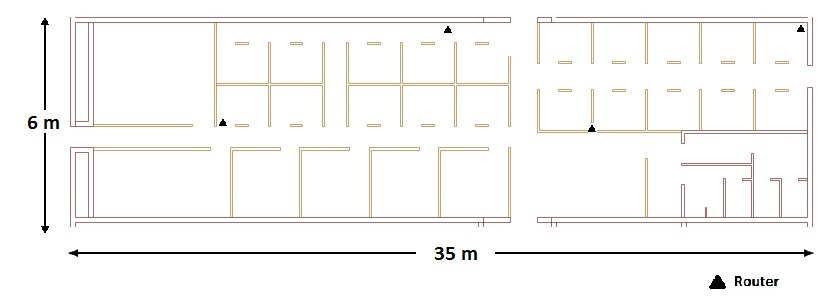
\includegraphics[width=135mm,height=50mm]{environment1.jpg}
\caption{Map of environment 1}
\label{fig:tenv1}
\end{figure*}

\begin{figure*}[!ht]
\centering
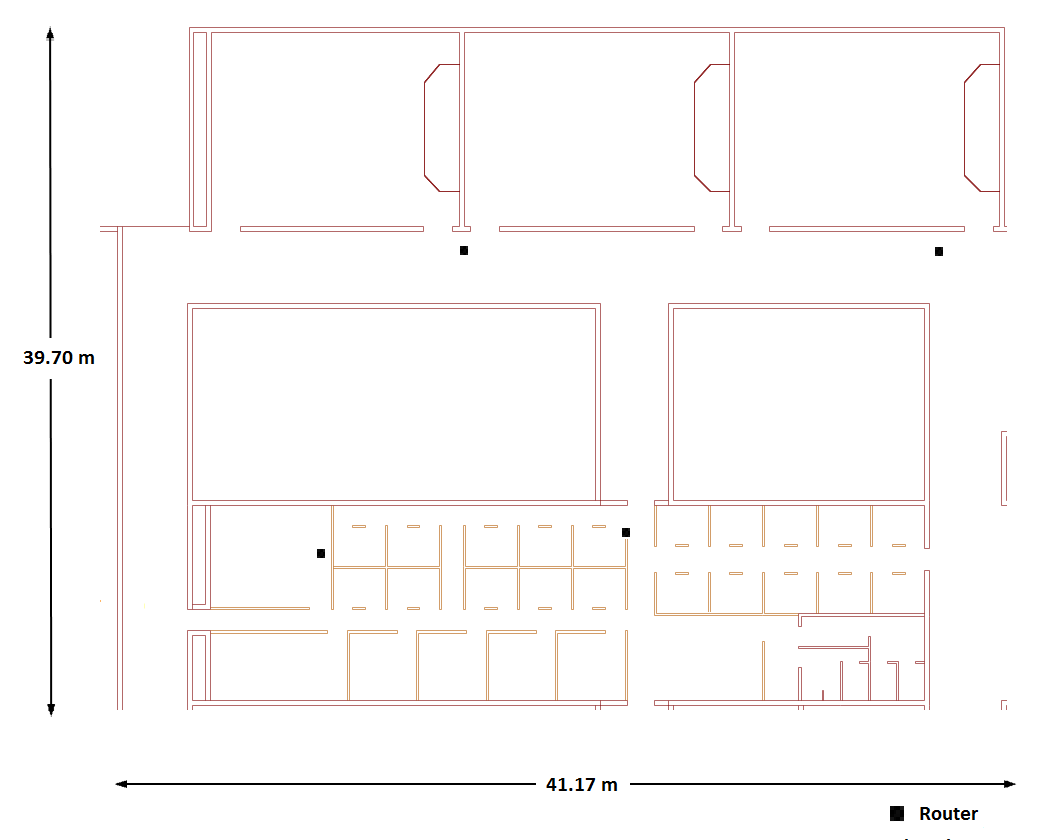
\includegraphics[width=135mm,height=70mm]{temp.PNG}
\caption{Map of environment 2}
\label{fig:tenv2}
\end{figure*}

\section{\textbf{Analysis of Trilateration}}

As discussed in previous sections, it is important to develop non-fingerprinting based solutions over trilateration for indoor localization. A suitable candidate for this is trilateration, which is a basic non-fingerprinting approach that is robust and easy to implement which however, suffers from poor accuracy. Towards this, we have analyzed the performance and patterns in trilateration and identified the potential areas for improvement and this section goes into the details of this analysis.

First, we discuss the target environment where we conducted our experiments to analyze the performance of trilateration. The target environment is a typical university space with office spaces, classrooms, and open areas, and is shown in Figure \ref{fig:tenv2}. It is a 41m x 38m space with wide passageways to walk around and includes several classrooms. It subsumes a large room 35m x 6m (\ref{fig:tenv1}) that is analogous to an office space with several cubicles, conference rooms, private rooms, and pathways. This large room serves as our first environment whereas the larger area is considered as our second environment to check the veracity of our experiments with a sparser router density.

Commercially available dual-band routers were placed in these environments. To achieve the optimal coverage of the area, the routers are strategically placed such that the variance amongst them is maximum \citep*{shanmugaapriyan2014pragmatic, kaemarungsi2012analysis, CiscoLocation}. To eliminate any shadowing due to obstacles, the routers were placed at a height of 2.43m \citep*{shanmugaapriyan2014pragmatic}, which aids in maintaining a line of sight with minimum path loss at each point. Thus the routers were positioned as shown in Figure \ref{fig:tenv1}.

Several experiments have been conducted in this environment, both for fingerprint data collected over multiple iterations\citep*{shanmugaapriyan2014pragmatic} and for performing calibration free localization. Additionally, experiments were performed to understand the path loss in different environments. Our analysis of the trilateration was conducted over several sample points in these data-sets where trilateration was performed and the overall accuracy was calculated. On probing the results, it was observed that for the majority of the points, the intersection region was inaccurate. Hence, a non-linear least-square regression was applied to find the probable region better and an average accuracy of 7.76m, with it being .64m in the best case and a poor 21.49m in the worse case scenario was observed. 

The accuracy definitely needs improvement, therefore warranting further analysis. Upon further examination, it was discerned that the source of this discrepancy could be attributed to the error in distance estimation based on distance propagation models. Hence, we consider many of the widely accepted propagation models and identify commonly associated problems with them. And  choose an appropriate one for our case. Models such as Okamura-Hata, Log-distance path loss, ITU \citep*{seybold2005introduction} are widely accepted and are derived from the free space path loss model, which originates from the inverse square law and the antenna gain.
Models such as  etc. are dependent on the log-distance equation to model the signal path loss \citep*{sarkar2003survey, soorty2015finding}.  For our experiments, we consider the log-distance path loss model as our RF propagation model \citep*{sarkar2003survey, soorty2015finding}.
\begin{equation}
\Bigg[\frac{P_{L}(d)}{P_{L}(d_{0})}\Bigg]_{dB}  ~=~ -10n log\Bigg(\frac{d}{d_{0}}\Bigg) + X_{dB}
\label{pathlosseqn}
\end{equation}
where $PL(d0)$ is the total path loss measured in (dB) at a distance d0, $PL(d)$ is the total path loss measured in (dB) at the distance d1, n is path loss exponent (3 in our case) and 'X' is equated to 0 usually.

While the log-distance path loss model takes shadowing into account, it still is founded upon empirically derived evidence and does not hold good in all environments. Shadowing is the effect that the received signal power fluctuates due to objects obstructing the propagation path between transmitter and receiver. The path loss exponent is an important parameter and not choosing an appropriate value could considerably alter the end results \citep*{srinivasa2009path}. Furthermore, the path loss exponent is prone to change with changes in the environment and is also affected by the obstacle density in a room.

It can be observed that a higher path loss exponent provides for better distance estimation in cluttered indoor spaces, but is prone to underestimations when the obstacles do not completely affect the line-of-sight. Lower path loss exponents are better in near-line-of-sight environments, but prone to overestimation in the presence of obstacles like walls. 

Identification of these errors is difficult since it is prone to environmental factors such as the humidity, temperature, and dynamically moving obstacles. In addition to these, they're also dependent on the receiver's line of sight to the router, the number of people in the room and their walking patterns. However, it is possible to identify the type of issues causing these errors by observing the trilateration itself, i.e. by observing the geometric patterns of the circles used in trilateration.

The subsequent paragraphs explain our observations and how they are characterized. These patterns can be made sense of only when standard guidelines are followed for optimally placing routers and the path loss exponent is decided after careful consideration. Any errors that occur due to bad placement or poor density of routers is beyond the scope of this work. Hence our observations are based on the adherence to these requirements. 

\subsection {\textbf{Key Observations in Trilateration}}
Our goal here is to identify the ramifications of these earlier mentioned factors on trilateration and methods to alleviate the error, and not the factors themselves. To better understand the cause of the errors, geometric patterns of the circles and their impact on the accuracy have been observed. Taking that into consideration, the patterns in the overlapping circles have been analyzed. Consider the three circles $c1, c2$, and $c3$ in the trilateration with radius $r1, r2$ and $r3$ respectively. Our primary observations are as follows:
\begin{enumerate}
    \item Underestimation can be understood from the trilateration pattern based on the level of overlap. 
    \item  Overestimation can be discerned for some cases based on the level of overlap
    \item From the strength of RSS and trilateration patterns, it can be determined if trilateration is the best approach for estimating a given point. 
     \item Due to estimation errors, it is important to give higher probability to the positions closer to the boundary of the circle containing the original point than the center.
\end{enumerate}
The following paragraphs will explain these observations in detail. 

As mentioned earlier underestimation occurs when estimated distance using the log-distance model is lower than the actual distance from the router, and is common in indoor scenarios. When observing the overlap of circles during trilateration, underestimation can be clearly determined when there is lack of overlap of some or all circles with other circles as defined below:
\begin{definition}{UnderEstimation}
If $c1 \cap c2 = \emptyset$  $||$  $c1 \cap c3 = \emptyset$  $||$  $c2 \cap c3 = \emptyset$ then $UnderEstimation = true$  
\label{def:under}
\end{definition}
When there is no overlap, resizing of circles is required so that overlap occurs. This distance re-estimation will be discussed in the next section. 
In the environments where the experiments were conducted, we have observed that from around 80 points that were evaluated, 57\% of them had underestimation. Figure \ref{types_underest} depicts different types of underestimation as observed from the fingerprint dataset collected in Environment 1. 
\begin{figure*}[t]
\centering
%\captionsetup{justification=centering}
\begin{tabular}{ |c|c|c| }
\hline
Two circle intersection & Relative intersection of & No Intersection \\
& two circles & \\        
\hline
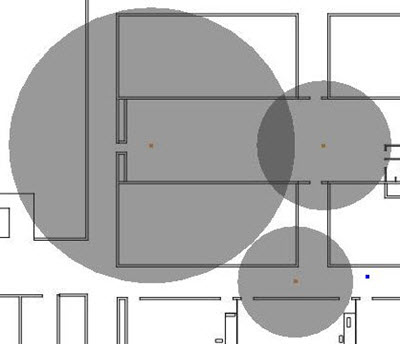
\includegraphics[width=0.28\textwidth, height=40mm]{Two-Intersect.jpg}
& 
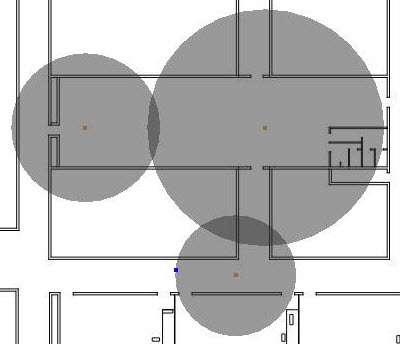
\includegraphics[width=0.28\textwidth, height=40mm]{In-Between.jpg}
& 
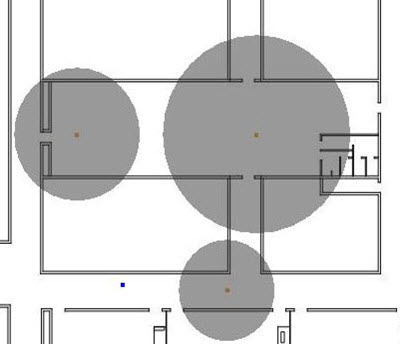
\includegraphics[width=0.28\textwidth, height=40mm]{Non-Intersect.jpg}
\\  \hline
61\% of the cases & 1\% of the cases & 38\% of the cases
\\ \hline 
\end{tabular}
\\
\hfill \break
\caption{Underestimation Patterns}
\label{types_underest}
\end{figure*}
\\

\textbf{Characterizing Overestimation:} Overestimation is usually observed when the trilateration circles are large, resulting in a larger overlapping region. While there are several possible cases that indicate overestimation, many of these need not necessarily mean so. When the point is close to one router for instance, the circles from other two routers usually tend to be large and have high overlap. This does not necessarily indicate overestimation, and several such factors can lead to patterns seemingly representing overestimation. However, in two types of overlap of the circles, we can be confident of overestimation. When a circle completely encloses another circle overestimation can be deduced. Additionally, overestimation can also occur when the percentage overlap between two circles is greater than a predefined threshold, and the third circle is not disconnected from the others. These cases are defined as follows

\begin{definition}{Overestimation}
Case 1: If $c1 \cap c2 = c1$ $||$ $c1 \cap c2 = c2$ $||$ $c1 \cap c3 = c1$ $||$ $c1 \cap c3 = c3$ $||$ $c2 \cap c3 = c2$ $||$ $c2 \cap c3 = c3$ then  $OverEstimation1 = true$ \\
Case 2: If $(|c1 \cap c2| > \delta$ $||$ $|c1 \cap c3| > \delta$ $||$ $|c2 \cap c3|>\delta)$ and $Underestimation = false$ then $OverEstimation2 = true $
\label{def:over}
\end{definition}

In both these cases, overestimation occurs mostly in the largest circle(s) and their radii have to be reduced proportionately. Based on our experiments in Environment 1, we observed few cases of overestimation. However, more cases are seen in the larger environment and around 19.5\% of the points have been overestimated. Our system detects every case of underestimation and overestimation that is clearly and accurately characterizable, but does not deal with fuzzy cases, and that is beyond scope of this work. 

\textbf{Trilaterability of a point:} When the receiver is near a router, its signal strength is usually high. However, since the circle is very small, and the distance is far from the other routers, the circle overlap is skewed and the trilateration area is rarely close to the point. 
Additionally, issues in error estimation as mentioned above complicates the overlap, leading to major localization errors. In such cases, it is observed that one circle is relatively much smaller compared to the other circles. When this circle is an overestimation, the point is inside the smallest circle and if it is an underestimation, the point is generally outside of all three circles, and resizing may not help much. In some cases, the points are positioned such that they  away from the influence of other two routers. These cases can be seen in Figure \ref{collageofpoints}. Classifying such points as non-trilaterable can help choose other techniques to estimate positions. In Environment-1 around 43\% of the points fall in this category and therefore must be identified and addressed differently. It must be noted that there are cases where trilateration can work for such cases. However, when not addressed specially, the accuracy is not affected drastically as we shall see in section 5.

\begin{figure}[t]
\centering
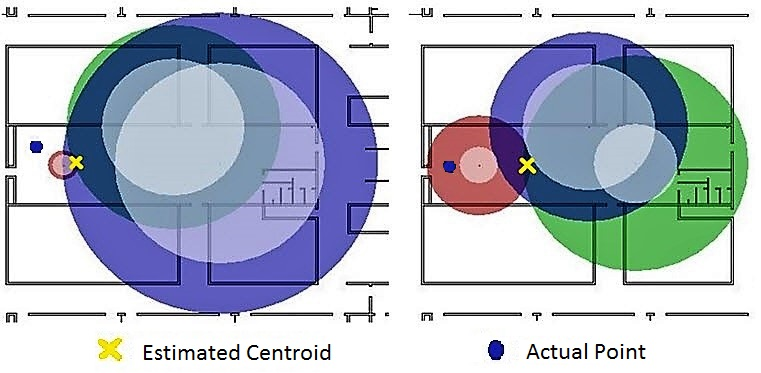
\includegraphics[width=84mm]{Anomalous_Centroid_Edited.jpg}
\caption{ Trilaterability of a point}
\label{collageofpoints}
\end{figure}

\textbf{Anomalous Centroid Position:} When trilateration occurs, the estimated point is the centroid of the overlapping area of the three circles. If the overlapping area (either after resizing or before) is high due to errors discussed above, it is possible that the estimated point is located more towards the center of any circle. When underestimation or correct estimation occurs, the point lies in the area around the border of one of the underestimated circles. If an overestimation occurs, the point may lie very close to the middle band of the circle. It is rare that the final point lies in the center of any disk and usually this occurs in the case when the point is very close to a router as discussed above. The figure \ref{fig:collageofpoints1} illustrates these cases. During trilateration, if this is accounted for, accuracy in estimation can be improved.
\begin{figure}[t]
\centering
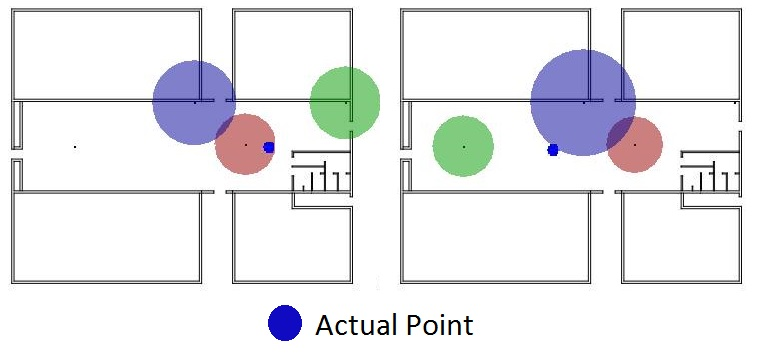
\includegraphics[width=84mm]{Skewed_Centroid.jpg}
\caption{Anomalous centroid }
\label{fig:collageofpoints1}
\end{figure}

In this paper, we use these findings to propose a Weighted Adaptive Location Estimation (WALE) algorithm that combines a probabilistic weighting approach with a dynamic circle resizing approach. The algorithm is customized based on whether a point is trilaterable or not. The next section will explain our algorithm in detail. 
\section{\textbf{Weighted Adaptive Location Estimation}}
In this section we discuss the details of our proposed algorithm and the outline of the weighted adaptive location estimation algorithm is as follows. 
\begin{itemize}
   \item For a given point, the distances to the three nearest routers are estimated using the log-distance model shown in Equation \ref{pathlosseqn}. As explained in the previous section, based on the overlap, and the strength of the signal we can determine if there is underestimation or overestimation. 
  \item Depending on the property of the overlapping circles, distance is re-estimated i.e., the circles are enlarged or made smaller appropriately using a novel distance re-estimation algorithm.
  \item If the strength of a router is much higher than the other two as defined in the previous section, then it is better not to trilaterate.
  \item An appropriate weighting function is applied across the radius of the circle to estimate the probability of a point lying at any potential distance from the center depending on whether underestimation or overestimation has occurred. 
  \item Using this function customized to the trilaterability of the point, we design an algorithm that calculates the maximum likelihood position.
\end{itemize}
We now delve into the details of the algorithm and discuss the first step of distance re-estimation next. 

\subsection{\textbf{Distance Re-estimation}}

%\vspace{0.3in}
\begin{table}
\centering
\begin{tabular}{ | c| c| c| c| c| } 
\hline
Routers &A &B &C &D \\
\hline
Percentage of Points & 74 & 77.90 & 73.34 & 83.34 \\
\hline
\end{tabular}
%\vspace{0.3in}
\centering
\caption{Correlation of lower RSS with lower errors}
\label{lower-rss}
\end{table}

The RSS signals received from the routers is used to calculate the distances based on the log-distance model. However, the calculated distances may not be perfect and can be influenced by underestimation or overestimation (see Definitions \ref{def:under} and \ref{def:over}). This results in errors in estimating the position, and therefore a re-estimation of the radii of the three circles is necessary. We design a distance re-estimation algorithm that resizes the circles either by increasing or decreasing the radii as needed. It works on the following principles: 

\begin{enumerate}
\item When RSS is strong, its trustworthiness is high, but it is not completely error free, so resizing should be minimal for that router. This is also evident from previous experiments that the error occurring is indirectly correlated with the value of RSS \citep*{chandrasekaran2015inplace}. In addition, the same conclusion can be evinced from the experiments performed wherein 77.14 \% of the points that were close (less than 3m) to any of the four routers exhibited lower error rates as can be seen in Table \ref{lower-rss}.
\item When two circles are close to each other or nearly intersecting, it can either indicate data from two reliable routers or errors which are difficult to determine. Therefore their radii should be minimally increased. 
\item When a circle is overestimated, its radius should be reduced first before addressing the other circles. This allows for a better circle resizing in the subsequent phase. 
\end{enumerate} 

Based on our findings, we propose the following algorithm.

\begin{enumerate}
    \item We first begin by sorting the RSS values obtained from each of the routers. The smallest of these values is increased the least. The two other circles are increased accordingly. 
    \item In a round robin fashion, we check for circle intersection after each iteration of increase. If intersection is detected, the increasing algorithm stops for the circle that intersects with one of the other circles. When two circles are in close proximity, their rate of increase should be minimal. This is achieved by stopping the resize of any circle once it intersects with another circle. 
    \item In the case of overestimation, the radius of the larger circle is iteratively reduced such that intersection doesn't happen. Subsequent to this case, Steps 1 and 2 are performed.
\end{enumerate}

Consider an array of circles $C$, which are sorted in decreasing order of radius, and a queue $Q$ used as a temporary data structure. Each circle $c_i \in C$, is defined by the original radius $r_i$ and the re-estimated radius $r_i'$.  $r_i'$ is same as  $r_i$ initially. The algorithm for resizing the circles is given in \ref{CRalgo}. 
The algorithm \ref{DRalgo} using the definitions \ref{def:under} and \ref{def:over}, determines if the point is underestimated or overestimated and the algorithm directly implements the definition. It first accounts for case 1 of overestimation and reduces the encompassing circle appropriately. If this property does not hold, it checks for underestimation and if that fails, the second case of overestimation is checked. To address underestimation a cyclic increase algorithm is developed as given in \ref{CRalgo}. 

\begin{algorithm}[!ht]
\SetAlgoLined
\KwResult{Circles with a smaller intersection region}
\uIf{OverEstimation.Rule(1)==true}
{
	$r_1'$ = $dist({c_1,c_2}) - r_2' $\;
	$CyclicIncrease()$ \; 
} 
\uElseIf{UnderEstimation == true}
{
	$CyclicIncrease()$ \;
}
\Else{
	\If{OverEstimation.Rule(2) == true}
	{
		\While{OverEstimation.Rule(2)==true}
		{
			$r_1' = r_1' - \beta * r_1$ \;
			$r_2' = r_2' - \beta * r_2$ \;
		}
	}
}
\caption{Distance Re-estimation Algorithm}
\label{DRalgo}
\end{algorithm}
The cyclic increase algorithm works as follows. A queue Q is initialized with the circle indices in decreasing order of radii. The algorithm starts by dequeuing the largest circle and its radius is compared with that of the next two circles. If the circle overlaps with other two circles, then no further increase or decrease to radius will happen to the circle. The function $overlaps$ checks for overlap and whether they overlap by 5\%. However, if the circle does not intersect with both of the other circles, then its radius is increased by $\beta$ \%. The above steps are repeated for the subsequent larger circles. This increase occurs cyclically for all the three radii until the circles overlap favourably. Here $\beta$ is set experimentally.
In the case of overestimation, the algorithm first checks for complete encompassing of circles. When this is detected, the algorithm reduces the radius of the encompassing circle such that the circles are adjoining and the cyclic resizing algorithm is applied. In the event of the overlapping region being too large, as defined in section 3, the largest circle's radius is reduced with the same constraints as stated above. $\delta$ is also set experimentally.
\begin{algorithm}[!ht]
\SetAlgoLined
\KwResult{Resized circles with meaningful intersection region}
\While{!Q.isEmpty()}
{
	i=Q.front()\;
	\If{($c\_i.!Overlaps(c\_{i+1} mod 3$)) $||$ ($c\_i.!Overlaps(c\_{i+2} mod 3$))}
	{
		$r\_i'$ $\leftarrow$ $r\_i'$ + $\beta$ * $r\_i$; \\
	    Q.enQueue(Q.deQueue());

	}
	\Else{
	        Continue;
	    }
	
}
\caption{Cyclic Increase Algorithm}
\label{CRalgo}
\end{algorithm}
\vspace{-0.2in}
\subsection{\textbf{Classification of Non-Trilaterable Points}}
Before estimating the position, we classify each candidate point $p$ as trilaterable or not. The ratio of the smallest circle to the next larger circle is checked and if it is less than $\alpha$, then this point will not lie in any overlapping region of the circles even after re-estimation, and therefore is not trilaterable. Whenever the router has a strong RSS and there is a combination of underestimation and overestimation, the likelihood of an estimated point lying in an overlapping region even after re-estimation is low. In this case, trilateration will yield a huge localization error and hence the estimation of these points is done differently. 
 
To estimate $\alpha$, a sample set of points from a region is taken, and their distances to the closest three routers are estimated. The ratios are calculated and the median of the frequency distribution of these ratios gives a potential estimate for $\alpha$. We have observed that this method of determining $\alpha$ works reasonably well for different environments.

\subsection{\textbf{Weighted Position Estimation}}

After classifying the candidate point $p$ as above, the location of $p$ is estimated by a novel weighting algorithm which is explained in this section. Firstly, a weighted occupancy grid is overlaid on the region of interest. The weight is calculated for every radius $k$ varying from $0$ to $r_i'$, therefore the weight is uniform for every point along the circumference of a circle with radius $k$.

Weights are calculated for each classified distance using the equation:
\begin{equation}
W[k] = \frac{1}{r}  e^{\frac{k}{r}}    
\end{equation}

The weighting follows an exponential function, and gives higher weighting to the points in the border of the circle and lower weights to points closer to the center.  It must be noted here that since overestimation occurs in very few cases, and level of overestimation is low, we use the same weighting function for overestimation. However when overestimation is high, we can use a log-normal distribution, with the median at around $3r/2$, were $r$ is the radius. Let $T$ be the trilateration region containing the points in all three circles.

\begin{algorithm}[!ht]
\SetAlgoLined
\KwResult{Location estimate of device}
\For{$i$ $\leftarrow$ 0 $to$ 2}
{
    \For{Each $k$ $\leftarrow$ 0 $to$ $r\_i'$}
    {
        $k$ $\leftarrow$ Distance(x,y,$c\_i$.centre()) ;\\
        $W[k]$ $\leftarrow$ (1/$r\_i$)*($e^{(k/r\_i)}$);\\
        \For{$j$ $\in$ $c\_i$ at distance $k$ from center }
        {   
            \If{$j$ $\in$ $c\_{(i+1)mod 3}$ $||$ $j$ $\in$ $c\_{(i+2) mod 3}$}
            {
                \If{p.isTrilaterable()}
                {
                    $j.weight$ $\leftarrow$ $j.weight$ + $W[k]$ ;
                }
                \Else
                {
                    $j.weight$ $\leftarrow$ $abs(j.weight - W[k])$ ;
                }
            }
            \Else
            {
                $j.weight$ = $W[k]$ ;
            }
        }
    }
}
\caption{Weighting Algorithm}
\label{Adaptive Weighting}
\end{algorithm}

The above weighting algorithm is applied to each circle. For the overlapping regions between circles, the weights are aggregated if the point is trilaterable, else the absolute difference between them is taken. When a point is trilaterable the overlapping regions are given higher weight-age. This is similar to trilateration; however, the weighting algorithm helps refine the likelihood area where the point could lie. When the candidate point is not trilaterable, it is essential to increase the likelihood of it lying in the smallest circle, while reducing the impact of the other routers. Therefore, in the case of overlapping regions, the weighting is reduced by taking the absolute difference of the individual weights. By doing this the point is pushed towards the smaller circle and away from the others. The WALE algorithm, by doing an adaptive weighting takes care of different cases that could occur, and helps improve accuracy.

\section{\textbf{Analysis and Results}}

In this section, we analyze the efficacy of our algorithm in comparison with other non-fingerprinting approaches and also delve into a detailed analysis of our algorithm. Our algorithm is implemented on a fingerprint dataset in Environment-1, and data collected by a localization experiment over random points across Environment-2. As explained in section 3, the first environment is a typical indoor office space with minimal shadowing. The second environment has semi-open spaces in between, which could increase the complexity of the environment but nonetheless, provide an insight into the robustness of the algorithm.

\begin{figure*}[!ht]
\centering
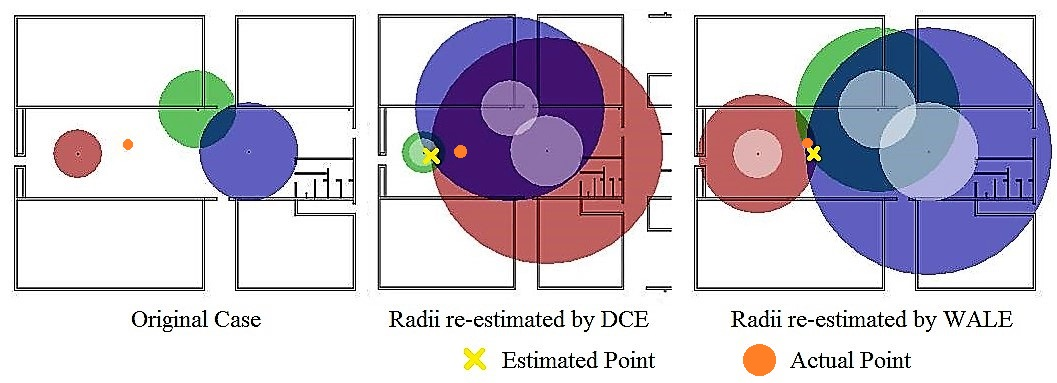
\includegraphics[width=125mm]{comparisoncase.jpg}
\centering\caption{WALE resizing vs DCE}
\label{re-est}
\end{figure*}

\subsection{\textbf{Performance of WALE}}
We first analyze the performance of WALE in the two environments. We juxtapose the results of our algorithm along with that of two other algorithms that we implemented. The comparison of the results is elicited in forthcoming paragraphs.
The two other methods that we implement are
\begin{itemize}
    \item Basic Trilateration with Simple circle increase
    \item Trilateration over Dynamic Circle Expansion (DCE) algorithm
\end{itemize}

We first test WALE against basic trilateration. Basic trilateration is applied to the circles after increasing the sizes of all circles by 10\% at every iteration till they meet. We also compare WALE with trilateration applied over DCE. 
We have proposed a cyclic distance re-estimation algorithm and have chosen it over the Dynamic Circle Expansion \citep*{DCE} to perform localization. We provide an empirical justification for this by comparing the accuracy of our approach over trilateration applied over DCE. 
In both these algorithms that we use for comparison, trilateration is not weighted and does not account for overestimation or non-trilaterable cases. Table \ref{my-label} presents the relative performance of the two algorithms in both these environments. 
In the earlier sections, we stressed the need to improve trilateration. Therefore, we compare WALE with basic trilateration or modified trilateration algorithms, as discussed in sections 1 and 2, because our focus is to determine the improvement in accuracy achievable using trilateration. Furthermore, there are several other methods that depend upon trilateration such as bluetooth, acoustic waves, etc.

\begin{table}[!ht]
\centering
\begin{tabular}{|l|l|l|l|}
\hline
Environment                                                              & WALE     & \begin{tabular}[c]{@{}l@{}}Basic\\ Trilateration\end{tabular} & DCE         \\ \hline
\begin{tabular}[c]{@{}l@{}}I - Average Error (in m)\end{tabular}        & 2.98 & 3.56                                                      & 3.55 \\ \hline
\begin{tabular}[c]{@{}l@{}}I - Std Deviation\end{tabular}  & 1.65 & 2.31                                                     & 1.81    \\ \hline
\begin{tabular}[c]{@{}l@{}}II - Average Error (in m)\end{tabular}       & 3.55   & 11.67                                                      & 4.90    \\ \hline
\begin{tabular}[c]{@{}l@{}}II - Std Deviation \end{tabular} & 2.41 & 8.53                                                      & 4.26    \\ \hline
\end{tabular}
\vspace{0.1in}
\caption{Overall Performance of WALE}
\label{my-label}
\end{table}


The results indicate that WALE performs much better than basic trilateration especially in Environment-2 which is more challenging and has both indoor and outdoor spaces. Even in a regular office environment WALE performs better. Our results indicate that even a simple circle resize may account for errors in some cases, it performs poorly in many cases (see standard deviation). Additionally, we observe that our algorithm performs better than DCE especially in Environment-2. In DCE, the smallest circle is fixed. However, if this is an underestimation, the error incurred is high and our algorithm by considering both the strength of routers and the level of overlap, works better. Figure \ref{re-est} demonstrates this for an example point, where our resize method accounts for underestimation in the smallest circle also. From the table, we also observe that our algorithm is more stable in both environments as observed by the low standard deviation. 

When we compare our circle resize algorithm with trilateration (without applying weighting or accounting for non-trilaterability) versus DCE with trilateration, we see that our approach performs better. In environment 1, our approach has an average error of 3.39, with a standard deviation of 2.25. However in environment 2, its average error is 4.824m with a standard deviation of 3.79. We observe that our algorithm performs better in hybrid environments where overestimation is more pronounced. Since DCE fixes the smallest circle and only increases the other two, it accounts for non-trilaterable cases to some extent and performs better in those cases, but its performance in other cases is not very good. Additionally,  this makes improving performance by considering trilaterability less probable. However when trilaterability and weighting is added to our resizing algorithm WALE outperforms other approaches, thus justifying the cyclic resizing approach. 
\subsection{\textbf{Analysis of the WALE Algorithm}}
Next, we analyze the operation of the WALE algorithm to determine how different components contribute to its accuracy. We also analyze how our observations and the solutions aimed at addressing them translate to accuracy in localization.
\begin{table}[!ht]
\centering
\begin{tabular}{|l|l|l|l|}
\hline
Environment                                                              & WALE     & \begin{tabular}[c]{@{}l@{}}Basic\\ Trilateration\end{tabular} & DCE      \\ \hline
I - Average error (in m)                                                   & 2.61 & 2.87                                                      & 2.62 \\ \hline
I - Std Deviation                                             & 1.38 & 1.83                                                      & 1.46 \\ \hline
\begin{tabular}[c]{@{}l@{}}II - Average error (in m)\\ \end{tabular}       & 3.18 & 5.49                                                      & 11.71 \\ \hline
\begin{tabular}[c]{@{}l@{}}II - Std Deviation \end{tabular} & 2.46 & 3.48                                                      & 7.34 \\ \hline
\end{tabular}
\vspace{0.1in}
\caption{Performance for Underestimation Points}
\label{underest-acc}
\end{table} 
\vspace{-0.3in}
\subsubsection{\textbf{Accounting for Underestimation}}
In both our environments, a larger percentage of underestimation cases have been detected and our cyclic re-estimation algorithm helps address this, while the weighted adaptive localization helps estimate the location accounting for this underestimation. The performance of our algorithm for the points that have a clear case of underestimation as defined in Section 3 is given in Table \ref{underest-acc}. In Environment-1 where there is primarily underestimation, we see WALE performing slightly better than the others, but a drastic improvement is seen in the larger and more complex environment. WALE's average accuracy and standard deviation are much better than the others. The combination of the cyclic increase of circle radii, along with weighted trilateration helps improve the accuracy. We see that DCE performs poorly in Env II, and this is due to its reliance on the strength of the strongest router. In complex environments, the strongest signal may not be reliable and other factors have to be considered, and these are the cases where our cyclic resize combined with the weighted location estimation works well. 
\begin{table}[!ht]
\centering
\begin{tabular}{|l|l|l|}
\hline
Environment                                                              & WALE     & \begin{tabular}[c]{@{}l@{}}Basic\\ Trilateration\end{tabular} \\ \hline
\begin{tabular}[c]{@{}l@{}}II - Average Error (in m)\end{tabular}       & 4.98  & 11.50                                                      \\ \hline
\begin{tabular}[c]{@{}l@{}}II - Std Deviation\\ \end{tabular} & 1.66 & 3.41                                                      \\ \hline
\end{tabular}
\vspace{0.1in}
\caption{Performance for Overestimation Points}
\label{overest-accu}
\end{table}

\subsubsection{\textbf{Accounting for Overestimation}}

As mentioned in Section 3, we characterize overestimation in two cases and there were a few points in the larger environment, while there was no clear-cut overestimation in Environment-1. From table \ref{overest-accu}, we can see that basic trilateration performs very poorly for such points and therefore, accounting for it is important. Thus our algorithm reduces the overall estimation error greatly. We also applied our algorithm to these points but did not treat them as overestimation and estimated the average error, which turned out to be 5.105m. This can be attributed to a low incidence of overestimation and the level of overestimation is not too high to impact accuracy. However, we believe our algorithm will provide higher accuracy margins for stronger overestimation cases. 

\subsubsection{\textbf{Addressing Trilaterability}}
\begin{table*}[t]
\centering
\begin{tabular}{ |c|c|c|c|c|c|c|c| } 
\hline
$\alpha$ & 0.4  & 0.45 & 0.5 & 0.55 & 0.6 & 0.65 & 0.7 \\
\hline
Accuracy & 3.23 & 3.10 & 3.05 & 2.98 & 3.07 & 3.12 & 3.21 \\
\hline
\end{tabular}
\vspace{0.2in}
\caption{Accuracy of WALE with varying $\alpha$}
\label{alpha-types}
\end{table*}
One of our primary hypothesis was that certain points are better off when trilateration is not applied due to the nature of these points. We defined that when the ratio of the smallest circle radius to the next largest is lesser than $\alpha$, it is better not to trilaterate. We used a different weighting for these points as discussed in Section 4 so that trilateration based location estimation does not occur. Firstly, it is essential to determine the value of $\alpha$. Theoretically, we define it as the median of the frequency distribution of this ratio of sample points in an environment, which came to 0.55 for Environment-1. Experimentally, we verify this by calculating WALE's average error for different values of $\alpha$ as seen in Table \ref{alpha-types}, and we observe that the value with the best performance is close to the estimated value of $\alpha$. 
Using this empirically determined $\alpha$ value we need to answer the following questions. For those points which we consider as not trilaterable, what accuracy does the non-trilateration based algorithm provide? Are there points where trilateration would have been a better solution and if so how much accuracy is compromised? On an average, we see that the non-trilateration based algorithm provides an error of 3.269m in Environment-1 and an error of 4.874m in the larger Environment-2. If weighted trilateration was done on these points the error would have been 4.151m and 7.388m respectively. This demonstrates the need to address these points differently. From table \ref{wale-types} we observe that though there are cases where trilateration still works, the accuracy compromised is not as high as not treating these points as non-trilaterable. However, better solutions for such points is desirable and is part of ongoing work.
\begin{table}[t]
\centering
\begin{tabular}{|c|l|l|}
\hline
\multicolumn{3}{|c|}{Environment - I}                                                           \\ \hline
\multirow{2}{*}{$\alpha$ \textless 0.55}                       & Gain in Accuracy & 2.42 \\ \cline{2-3} 
                                                               & Loss in Accuracy & 2.20 \\ \hline
\multicolumn{3}{|c|}{Environment - II}                                                          \\ \hline
\multicolumn{1}{|l|}{\multirow{2}{*}{$\alpha$ \textless 0.60}} & Gain in Accuracy & 5.76     \\ \cline{2-3} 
\multicolumn{1}{|l|}{}                                         & Loss in Accuracy & 3.58    \\ \hline
\end{tabular}
%\vspace{0.1in}
\caption{Weighted Trilateration vs Non - Trilateration}
\label{wale-types}
\end{table}
%\vspace{-0.3in}
\subsubsection{\textbf{Impact of Weighted Trilateration in WALE}}
To verify the contribution of our weighting function to the increase in accuracy, we compare WALE against just trilateration applied over our distance re-estimation algorithm. We see that both the accuracy and stability in localization is improved by performing weighted location estimation over basic trilateration as seen from table \ref{imp-weighting}. This supports our hypothesis that the probability of a point lying towards the outer regions of the circles is higher than towards the center. Therefore, accounting for the error in estimation helps improve accuracy. 
\begin{table}[!ht]
\centering
\begin{tabular}{|c|c|c|}
\hline
Environment         & WALE   & \begin{tabular}[c]{@{}l@{}}Trilateration after \\     Cyclic Increase\end{tabular} \\
\hline
I - Average Error (in m)  & 2.98 & 3.39              \\
\hline
I - Std Dev   & 1.65   & 2.25                \\
\hline
II - Average Error (in m) & 3.55 & 4.824               \\
\hline
II - Std Dev  & 2.41   & 3.79             \\  
\hline
\end{tabular} 
%\vspace{0.1in}
\caption{Performance of Weighted Location Estimation}
\label{imp-weighting}
\end{table}
\vspace{-0.25in}
\subsection{\textbf{Discussion}}\
    From our analysis, there are a few key observations. Firstly, our distance re-estimation algorithm contributes greatly to improvement in localization. When the environment is challenging and prone to more errors in distance estimation, the contribution of our re-estimation algorithm is more significant. This improvement is not because of the refinement of the RSS data collected over the years in the area, but directly from the contribution of our algorithm that accounts for the errors in the distance estimation by addressing underestimation and overestimation. 
    Improvement in the localization accuracy, while it can be achieved by using a denser network of access points or by using specialized hardware, isn't always the feasible solution because it leads to increase in operating costs. Hence in our method, we try to focus on improving the accuracy by modifying the algorithm to better address problems that are commonly associated with performing trilateration.
    
    To our knowledge, this is the only approach that addresses both underestimation and overestimation. Additionally, it also contributes to the low variability in error which is an important aspect of localization. Secondly, the weighted location estimation helps reduce error to some extent and its significance is greater in more challenging spaces. Interestingly, classifying points as trilaterable or not actually contributes significantly to error reduction, and our approach to dealing with non-trilaterable points have worked well. Improving the performance of location estimation in these points can help improve accuracy even further. Since our algorithm is designed to address different types of errors, it can work in different environments and the improvement in accuracy would be dependent on the percentage occurrence of the types of errors and to the extent of these errors. Finally, we see that our algorithm has contributed to improving the stability of non-fingerprinting based localization as seen by the consistently low standard deviations across all cases.
    
\section{\textbf{Conclusion and Future Research Directions}}
    This paper proposed a novel weighted adaptive location estimation (WALE) algorithm that is a non-fingerprinting based approach for RSS-based WiFi localization. It takes into account both overestimation and underestimation errors and does an appropriate distance re-estimation such that the quality of trilateration is improved. Additionally, a novel weighted approach is used to estimate the likely position of the device. Our experiments over a regular office space and a larger and more complex indoor space, confirm that our algorithm provides better accuracies over other RSS based non-fingerprinting approaches. In addition, our algorithm has been empirically proven to be stable in different environments and under differing error scenarios. While the error has improved in many cases, better methods for accounting for overestimation and non-trilaterable points are needed. Machine learning based approaches can be used to identify and classify different types of localization errors and this is an area for future work.   

\begin{acknowledgements}
We thank Keshav Narayan and Vishal Chandrasekaran for their critical review of the draft of the paper and  students working at the Amrita Multi-dimensional Data Analytics Lab for their valuable support during the localization experiments. This work has been funded in part by DST(India) grant DyNo. C/4902/IFD/2016-2017. \end{acknowledgements}

\Urlmuskip=0mu plus 1mu\relax
\bibliographystyle{plainnat}
%\bibliographystyle{aps-nameyear}
%\bibliographystyle{spmpsci}
\bibliography{wifiref}
\nocite{*}

\end{document}


